\newpage
\section{Backups of simulations}
Very often when running a simulation you want to make a copy of it before continuing to play with the parameters.  To do this click on the backup simulation button in the database ribbon (see figure \ref{fig:database}), this will bring up the backup window, see figure \ref{fig:backup}. If you click on the "New backup" icon on the top right of the window, a backup will be made of your current simulation.  And an icon representing the backup will appear in the backup window.  To restore the backup double click on the icon representing your stored simulation. Note this backup is only stored in the your local simulation directory, and is more of a checkpoint than a real backup.... so make sure you have other copies of your simulation if it is very important to you..

\begin{figure}[H]
\centering
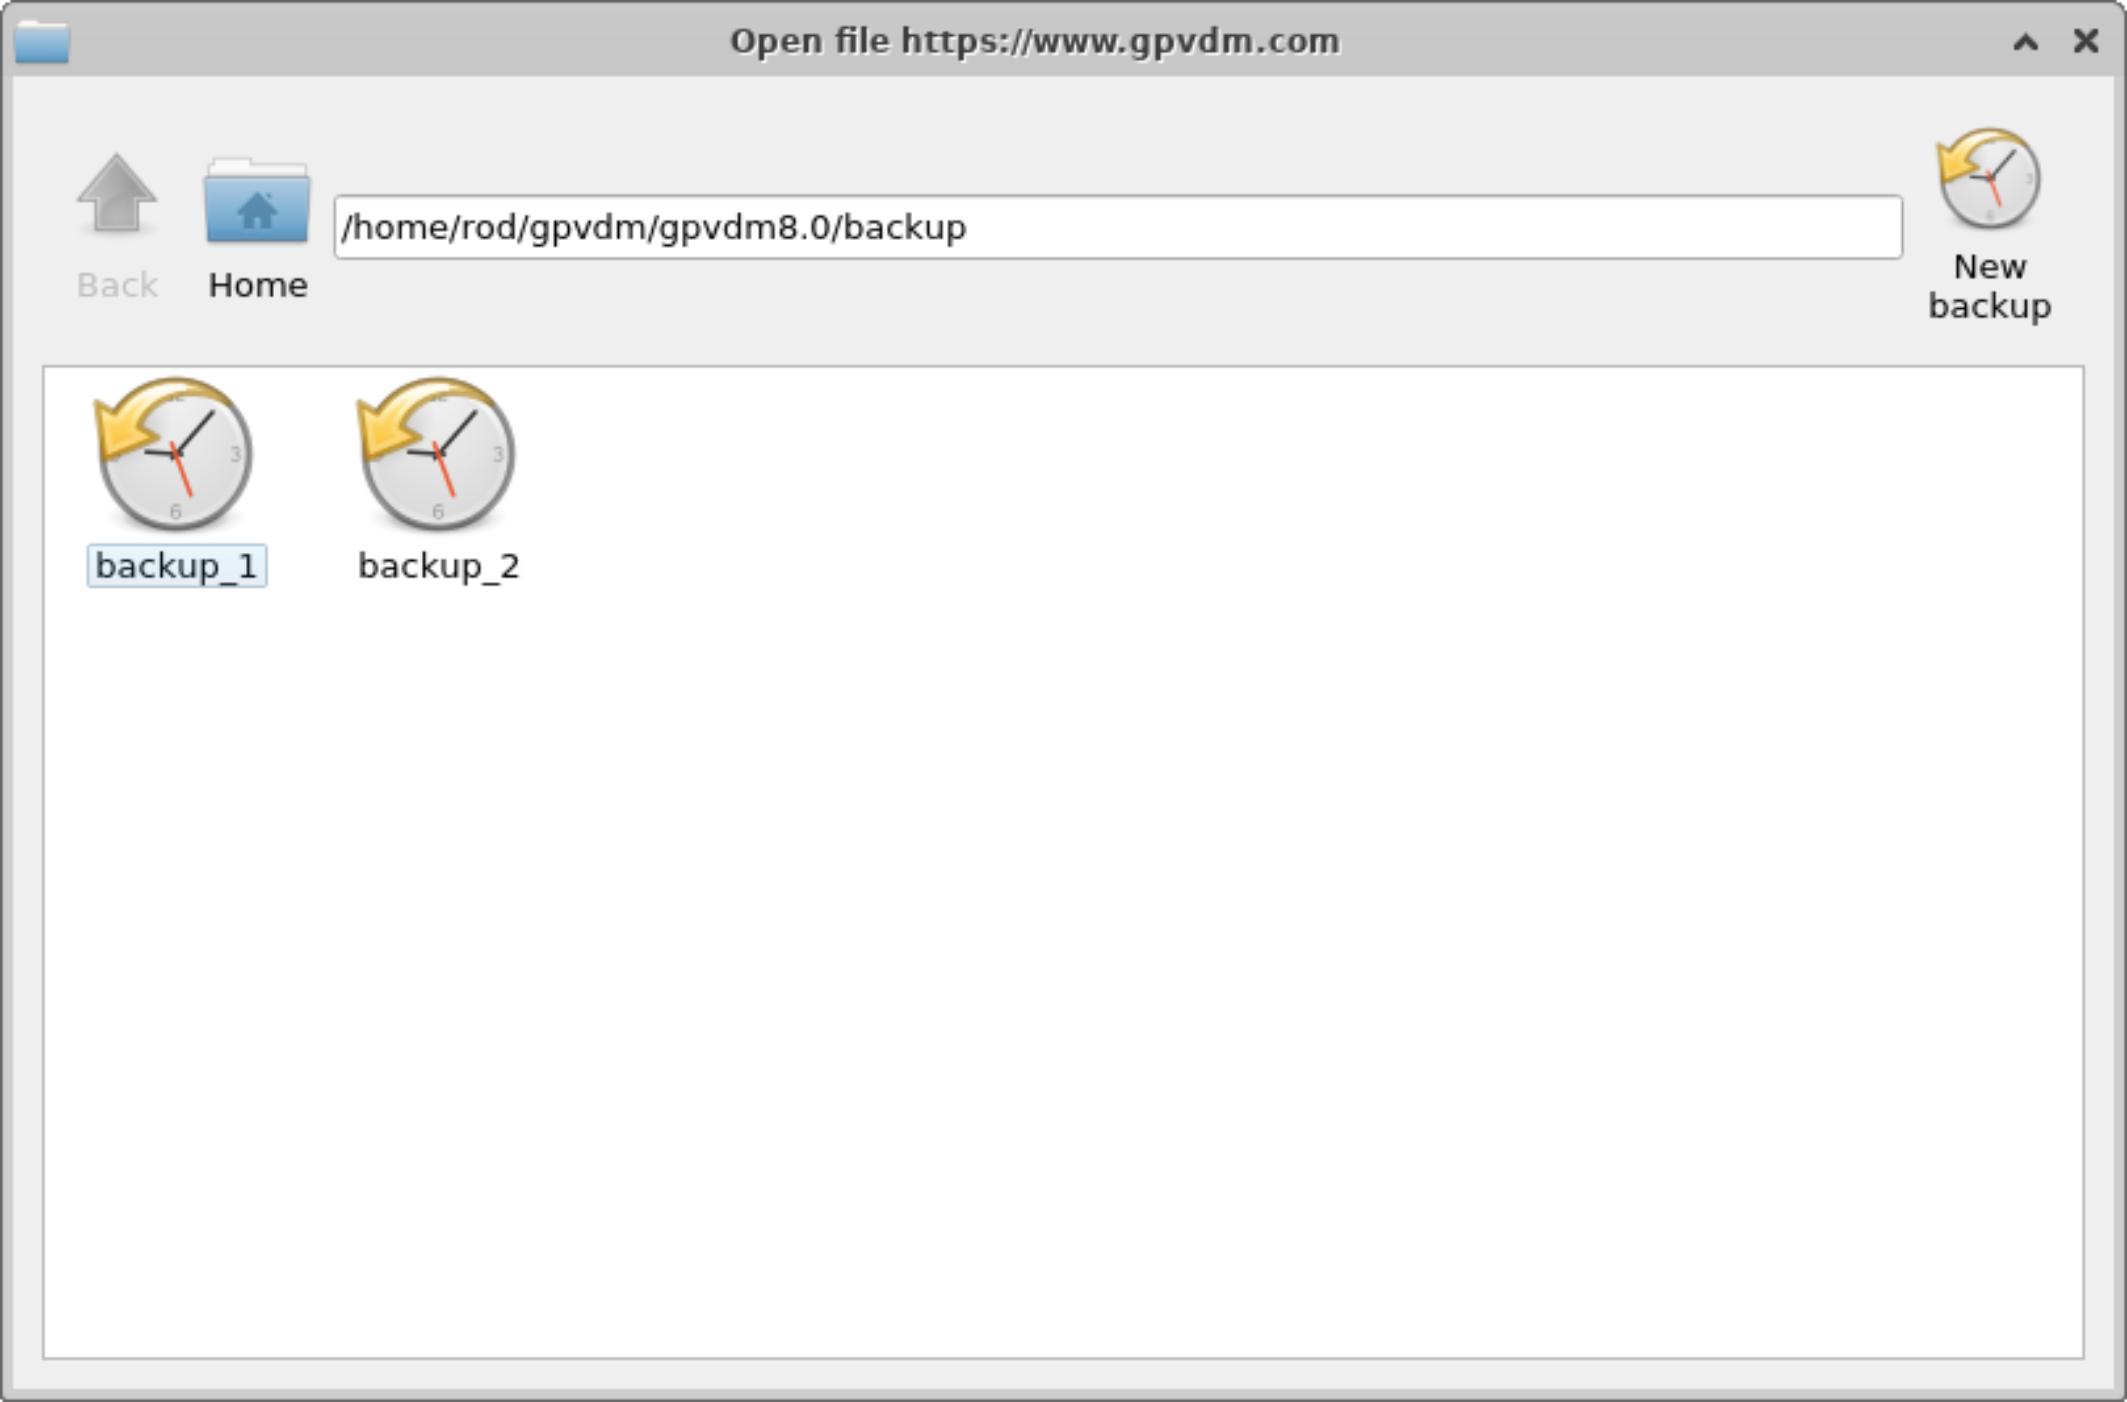
\includegraphics[width=0.7\textwidth]{./images/backup.png}
\caption{Backing up a simulation}
\label{fig:backup}
\end{figure}

